% !TeX spellcheck = en_US

\chapter{Introduction}
Nowadays it is very common in IT to have distributed systems in locations all over the globe\cite{1687567}. To provide the best user experience for the System administrators, it is important to monitor these networks by a few people sitting in remote locations. New approaches even try to automate the whole system so that it repairs itself. Important for the user in these systems is the availability and reliability of the system. 
\\
To tackle these tasks, Application Performance Management (APM) tools were build. They are available in a wide range of costs and qualities. They differ a lot in their architecture, features and style of approach to a problem. This is why we decided to make a comparison of some large Open-Source tool stacks available on the market. 
\section{Goals}
The Goal of the study is to print out the benefits and disadvantages of the popular Open-Source tools and stacks for monitoring available on the market. This could be from huge benefit for the new trend of DevOps(\cref{devops}) \cite{Bass:2015:DSA:2810087} . With a good monitoring tool, problems in the short intervals of deployment and testing offered by DevOps, could be identified more efficient. In special monitoring systems that log system internals in database, can be used in the debugging phase of an a agile development.  
\\ The work wants to illustrate the features and technologies of the tools to make it easier for the reader to get an overview of the different software approaches. In particular the tools will be tested in their ability to interact with modern cloud technologies like Docker and Kubernetes.\\
For these technologies, a good control mechanism that is customizable for every user can reduce the time to bug fix and the fear to develop the code.
 Furthermore, we want to take a look, on the ability of the stacks to integrate in existing environments and support of common tools and interfaces. Moreover, the cross compatibility of the stacks will be tested to the possibility of combining different tools in one environment. At the end a of the paper the reader should know which monitoring stack or which stacks are optimal for his or her environment.  

\section{Thesis Structure}
In the first part, the paper describes the general aspects of monitoring and how we split up tool stacks to take a closer look by the single responsibilities. This part also discusses the characteristics of the environments and their special interfaces. Here also an overview of our test environments is given. After the introduction, the tools will be introduced on their own. We first introduce the tools we actually tested in our study. After we list some tools we can't manage to install. As a conclusion to this work, a general overview  of the tool abilities in form of tables and an answer to the question of the best monitoring tools is given. This answer includes more than one tool because there a multiple option that fit on different purposes. Benefit here is that we can clearly exclude some tools out of the list in \cref{minimumrequire}, because they don't provide enough functions or there capability to integrate in a cloud environment is very poor.
\begin{description}
\item[Technical Data:] In this chapter, all technical aspects of the test environments and tools are discussed. Moreover, it provides our separation of the different APM activities. 
\item[Tools:] All tested tool stacks are listed and grouped by companies that developed and support them. If the stack consists of single tools that are usable in stand alone there is an extra section given that describes them and there interfaces. On the end of this chapter is a short list of tool we tested and were not able to deploy on a cluster.
\item[Evaluation:]The tested tools are compared in tables after there responsibility(Collector,Database,Visualization,Alerting). Here these tables we compare the statements of the provider with our experience of the tools.
\item[Conclusion:] Our experience with the tools and an answer to the question which stack is the best to use in cloud areas like Kubernetes.

\end{description}

\section{Minimum Requirements for the tools}
\label{minimumrequire}
In the process of searching for tool we set some minimum requirements that the tools have to fulfill, because over wise the amount of candidate for the study would be to big. The most important requirement was, that the tools are open-source. Moreover the tools had to be able monitor distributed systems and visualize the data. By the term distributed systems we  mean a micro service architecture. \\
In case that many of the tools had matched the requirements we defined so nice to have features. We preferred tools that were able to monitor web service over HTTP. Also tools that had an grouping function for alerts or can send the alerts over several interfaces. \\
At the end we had look at the following tools that all matched the minimum requirements of our study: TICK \cite{tick}, ELK Stack \cite{elk}, Prometheus \cite{prometheus}, Grafana \cite{grafana} \cite{grafana}, Zabbix\cite{zabbix}, Icinga\cite{icinga}, Cacti \cite{cacti}, OpenNMS \cite{opennms}, Munin \cite{munin}, Hawkular \cite{hawkular}, OpenTSDB \cite{opentsdb}, Zipkin \cite{zipkin}. Of this list we selected the first six tools to take a look on in our study.   


\section{DevOps}
\label{devops}
DevOps is a scheme for process improvement in the field of Software development and system administration\cite{Bass:2015:DSA:2810087}. It tries to improve the cooperation of both fields by shared process and tools.
By a agile style the process is visualized as a cycle \cref{fig:devopscycle} . Our study try's to improve the monitoring aspect of the cycle.
\begin{figure}
	\centering
	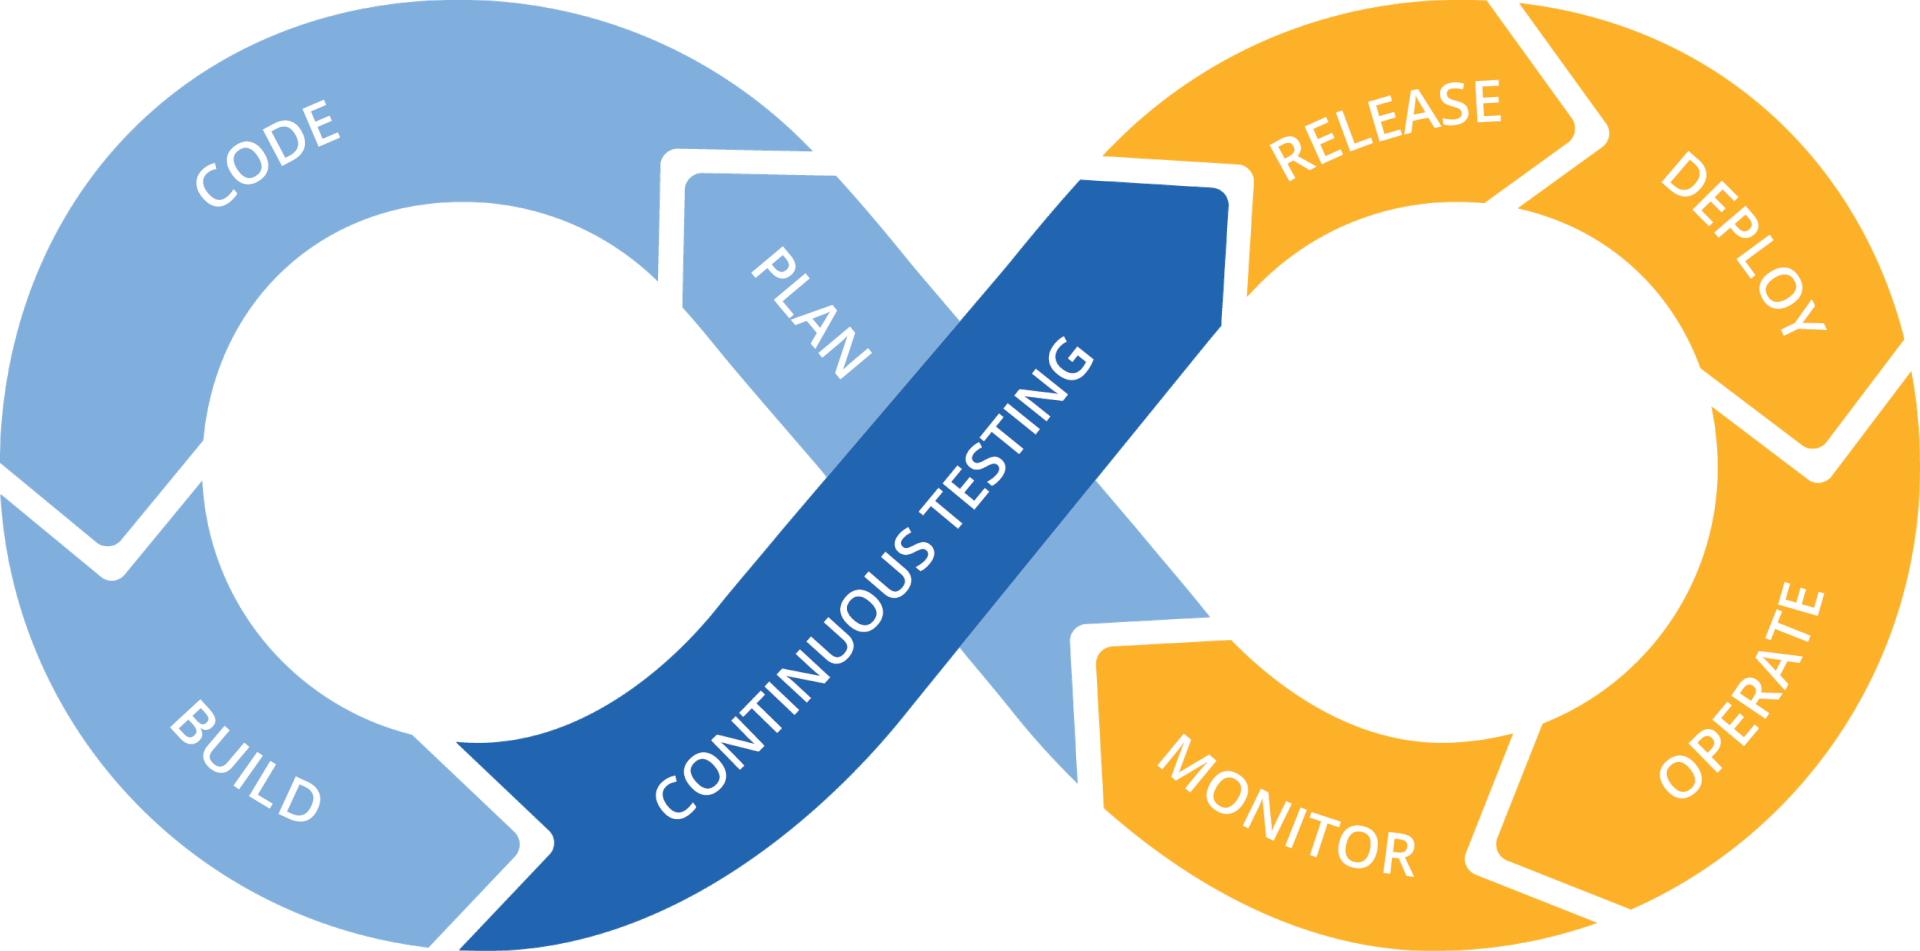
\includegraphics[width=0.5\textwidth]{Bilder/devopscycle}
	\caption{An example DevOpscycle}
	\label{fig:devopscycle}
	\cite{Devops}
\end{figure}